\documentclass[main.tex,fontsize=8pt,paper=a4,paper=portrait,DIV=calc,]{scrartcl}
% Document
\usepackage[T1]{fontenc}
\usepackage[dvipsnames]{xcolor}
\usepackage[nswissgerman,english]{babel}
\renewcommand{\familydefault}{\sfdefault}

% Format
\usepackage[top=5mm,bottom=1mm,left=5mm,right=5mm]{geometry}
%\setlength{\headheight}{\baselineskip}
%\setlength{\headsep}{0mm}

%\usepackage{scrlayer-scrpage}
%\clearpairofpagestyles
%\chead{{\bfseries\TITLE, \AUTHOR, \pagename~\thepage}}

%\addtokomafont{pagehead}{\upshape}

\usepackage{multicol}
\setlength{\columnsep}{2mm}
\setlength{\columnseprule}{0.1pt}

% Math
\usepackage{amsmath}
\usepackage{amssymb}
\usepackage{amsfonts}

% Code
\usepackage{fancyvrb, etoolbox, listings, xcolor}
%\usemintedstyle{bw}

%\newminted[shell]{bash}{
%fontsize=\footnotesize,
%fontfamily=tt,
%breaklines=true,
%frame=single,
%framerule=0.1pt,
%framesep=2mm,
%tabsize=2
%}
%\newminted{css}{
%breaklines=true,
%tabsize=4,
%autogobble=true,
%escapeinside=||,
%stripall=true,
%stripnl=true,
%}

    \definecolor{lightgray}{rgb}{0.95, 0.95, 0.95}
    \definecolor{darkgray}{rgb}{0.4, 0.4, 0.4}
    \definecolor{purple}{rgb}{0.65, 0.12, 0.82}
    \definecolor{ocherCode}{rgb}{1, 0.5, 0} % #FF7F00 -> rgb(239, 169, 0)
    \definecolor{blueCode}{rgb}{0, 0, 0.93} % #0000EE -> rgb(0, 0, 238)
    \definecolor{greenCode}{rgb}{0, 0.6, 0} % #009900 -> rgb(0, 153, 0)
    \definecolor{teal}{rgb}{0.0, 0.5, 0.5}

\lstdefinestyle{code}{
    identifierstyle=\color{black},
    keywordstyle=\color{blue}\bfseries\small,
    ndkeywordstyle=\color{greenCode}\bfseries\small,
    stringstyle=\color{ocherCode}\ttfamily\small,
    commentstyle=\color{teal}\ttfamily\textit\small,
    basicstyle=\ttfamily\small,
    breakatwhitespace=false,         
    breaklines=true,                 
    captionpos=b,                    
    keepspaces=true,                 
    showspaces=false,                
    showstringspaces=false,
    showtabs=false,                  
    tabsize=2,
    belowskip=-5pt
}



% Images
\usepackage{graphicx}
\newcommand{\pic}{\includegraphics[scale=0.3]}
\graphicspath{{Screenshots/}{../Screenshots}}
\makeatletter
\def\pictext#1#2{%
    \@ifnextchar[{%
    \pictext@iiiii{#1}{#2}%
    }{%
      \pictext@iiiii{#1}{#2}[0.5,0.4,0.3]% Default is 5
    }%
}
\def\pictext@iiiii#1#2[#3,#4,#5]{\begin{minipage}{#3\textwidth}\includegraphics[scale=#4]{#1}\end{minipage}\begin{minipage}{#5\textwidth}#2\end{minipage}}
\def\minipg#1#2{%
    \@ifnextchar[{%
    \minipg@iiii{#1}{#2}%
    }{%
      \minipg@iiii{#1}{#2}[0.3,0.6]% Default is 5
    }%
}
\def\minipg@iiii#1#2[#3,#4]{\vspace{0.8mm}\begin{minipage}{#3\textwidth}#1\end{minipage}\begin{minipage}{#4\textwidth}#2\end{minipage}{\vspace{0.8mm}}}
\makeatother

%\newenvironment{minty}[2]% environment name
%{% begin code
%  \begin{minipage}{#1}
%  \begin{minted}{#2}
%}%
%{% end code
%  \end{minted}
%  \end{minipage}
%  \end{minty}\ignorespacesafterend
%} 

% Smaller Lists
\usepackage{enumitem}
\setlist[itemize,enumerate]{leftmargin=3mm, labelindent=0mm, labelwidth=1mm, labelsep=1mm, nosep}
\setlist[description]{leftmargin=0mm, nosep}
\setlength{\parindent}{0cm}

% Smaller Titles
\usepackage[explicit]{titlesec}

%% Color Boxes
\newcommand{\sectioncolor}[1]{\colorbox{black!60}{\parbox{0.989\linewidth}{\color{white}#1}}}
\newcommand{\subsectioncolor}[1]{\colorbox{black!50}{\parbox{0.989\linewidth}{\color{white}#1}}}
\newcommand{\subsubsectioncolor}[1]{\colorbox{black!40}{\parbox{0.989\linewidth}{\color{white}#1}}}
\newcommand{\paragraphcolor}[1]{\colorbox{black!30}{\parbox{0.989\linewidth}{\color{white}#1}}}
\newcommand{\subparagraphcolor}[1]{\colorbox{black!20}{\parbox{0.989\linewidth}{\color{white}#1}}}

%% Title Format
\titleformat{\section}{\vspace{0.5mm}\bfseries}{}{0mm}{\sectioncolor{\thesection~#1}}[{\vspace{0.5mm}}]
\titleformat{\subsection}{\vspace{0.5mm}\bfseries}{}{0mm}{\subsectioncolor{\thesubsection~#1}}[{\vspace{0.5mm}}]
\titleformat{\subsubsection}{\vspace{0.5mm}\bfseries}{}{0mm}{\subsubsectioncolor{\thesubsubsection~#1}}[{\vspace{0.5mm}}]
\titleformat{\paragraph}{\vspace{0.5mm}\bfseries}{}{0mm}{\paragraphcolor{\theparagraph~#1}}[{\vspace{0.5mm}}]
\titleformat{\subparagraph}{\vspace{0.5mm}\bfseries}{}{0mm}{\subparagraphcolor{\thesubparagraph~#1}}[{\vspace{0.5mm}}]

%% Title Spacing
\titlespacing{\section}{0mm}{0mm}{0mm}
\titlespacing{\subsection}{0mm}{0mm}{0mm}
\titlespacing{\subsubsection}{0mm}{0mm}{0mm}
\titlespacing{\paragraph}{0mm}{0mm}{0mm}
\titlespacing{\subparagraph}{0mm}{0mm}{0mm}

%% format cells
\usepackage[document]{ragged2e}
\usepackage{array, makecell}
\renewcommand{\arraystretch}{2}
\newcommand{\mc}{\makecell[{{m{1\linewidth}}}]}



\lstset{
    language={[x86masm]Assembler},
    style=code,
}

\begin{document}
\begin{table}[h!]
\section{\textbf{Processor interaction}}
\begin{tabular}{|m{0.2\linewidth}|m{0.755\linewidth}|}
\hline
\mc{Memory-bus} & \mc{This enumerates the memory, as it can't be attached to the cpu directly, it would simply be a too long string.} \\
\hline
\mc{Data-bus} & \mc{This bus handles the data of a memory address that either has been read, or we want to write to.} \\
\hline
\mc{Control-Signals} & \mc{These indicate if we want to write or read.}\\
\hline
\mc{} & \mc{\textcolor{Red}{Note that the processor only really interacts with the rest of the system with the databus, the rest is only used in order to make the interaction happen at all!}}\\
\hline
\mc{\textbf{Instruction Set}} & \mc{A processor has a certain instruction set, that accesses it's own immediate register as well as request data from cache/memory. This is also the problem with Intel and AMD, they can't opensource their hardware properly as the instruction set is licensed by intel to other vendors. Therefore all hail Risc-V!} \\
\hline
\mc{} & \mc{Instructions are something like copy value of x into y, or write value u into p. But, there is also the instruction to simply do nothing!} \\
\hline
\mc{Sequence} & \mc{Just as the name says, it's a sequence of instructions to do something more specific than writing a value. Programs for example are just sequences of instructions. As we know, this is stored inside memory and is as stated above accessed by memory-bus.} \\
\hline
\mc{cache} & \mc{extremely fast but small memory insdide the processor.} \\
\hline
\mc{register} & \mc{Special datastructure inside the cpu that is even faster and smaller than the cache.} \\
\hline
\mc{Machine-Code} & \mc{The machine code is simply the encoding which the Sequences have to be in, in order for the CPU to understand the instructions. This is also why ARM programs do not run on an x86 system. The memory instructions would not be readable by the cpu. Rosetta is essentially just decoding and encoding these instructions.} \\
\hline
\mc{System-clock-cycle} & \mc{The entire system runs by the processor clock-cycle, it has 2 states, one constant sate, where values can only be read, and one change-able state, where any other operation can be done.} \\
\hline
\mc{Processor-cycle} & \mc{ 1. Processor orders the instructions from the memory with pointer.\\
  2. Processor decodes the Operation and Operands from the instruction.\\
  3. Processor chooses the corresponding core part (Baustein \#FuckGerman).\\
  4. Active Core might read from register.\\
  5. Active Core (part of it) executes operation.\\
  6. Active Core might write to register.\\
  7. Processor moves pointer according to operation size.\\
} \\
\hline
\mc{Encoding of Operations} & \mc{\pictext{2022-09-23-03:58:36.png}{The left side is a chain consisting of the Operation code and the register code. For example: the operation code \(1B_h\) will be combined with the register \(02_h\). This will combine like this in binary: \(011011_b\) append \(01\) -> \(01101101\) which is \(6D_h\) }[0.2,0.3,0.55]} \\
\hline
Little Endian Intel & Intel uses Little Endian due to certain benefits with this mode. \newline
\textbf{\emph{The biggest benefit is the fact that byte, word, dword all have the same address!}}\newline
\textbf{\emph{Remember from digicode, little endian is. \( s_1s_0\) \(s_3s_2\)}}\newline
\pic{2022-09-27-03:35:55.png}\\
\hline
Bit Byte and Word & Byte 8 Bit \newline 
Word 2 Byte / 16 Bit \newline
Doubleword 4 Byte / 32 Bit, or DWord \newline
Quadword 8 Byte / 64 Bit,or QWord \newline
Double Quadword 16 Byte / 128 Bit, or DQWord\\
\hline
Smallest Bit Count\newline
in the intel architecture & \textbf{The smallest amount that you can use in the intel architecture is 8bit}, in other words 1 byte. \newline You can't manipulate 1 single bit without taking 7 more with you.\\
\hline
\textbf{Register Formats} & \minipg{ 
In 16 bit architecture we have AH and AL registers, both being 8 bit.\newline
These accumulate to the \textbf{AX} Register.\newline
With 32 bit we get to \textbf{EAX} which extends the 16 bit by another 16 to the left.\newline
64 bit extends this further with another 32 and the name \textbf{RAX}.\newline
}{\pic{2022-10-04-03:34:45.png}}[0.5,0.5]\\
\hline
\end{tabular}
\end{table}
\pagebreak
\begin{table}[h!]
\begin{tabular}{|m{0,2\linewidth}|m{0.755\linewidth}|}
\hline
\emph{Further Terminology} & 
\minipg{
\begin{itemize}
  \item  \textbf{RAX} Accumulator for some operations, when none other is available
  \item  \textbf{RCX} Counter for loops or stringoperations
  \item  \textbf{RDX} Pointer for I/O Operations 
  \item  \textbf{RBX} Datapointer
  \item  \textbf{RSI,RDI} Source and Target-indices for stringoperations -> write your string to this
  \item  \textbf{RSP} Stackpointer, address for allocated stack
  \item  \textbf{RBP} Basepointer, address outside of stack, base for operation
  \item  \textbf{R8-R15} additional registers
\end{itemize}}
{\pic{2022-10-04-03:42:25.png}}[0.5,0.5]\\
\hline
\textbf{Length of Instruction} & 
\vspace{2mm}
\begin{itemize}
  \item Instructions are binary numbers which encode Operations and Operands
  \item Instructions can be 1-15 bytes long on the x86-64 architecture
  \item Count and size of parameters are dependend on the operation
  \item The length of an instruction is \textbf{not} included in the sequence
  \item A sequence must iterate through instructions to encode each instruction.\newline
  From start to finish.
  \vspace{-3mm}
\end{itemize}\\
\hline
\end{tabular}
\subsection{Operations}
\begin{tabular}{|m{0.2\linewidth}|m{0.755\linewidth}|}
\hline
\emph{Operations} & 
\vspace{2mm}
\begin{itemize}
  \item \textbf{Datatransfer Operations}
  \item \textbf{Arithmetic Operations}
  \item \textbf{Programflow Operations}
  \item \textbf{String Operations}
  \item \textbf{Operation for communication with the device}
  \item \textbf{Other Operations: Random Number Generator, Capability request}
  \vspace{-3mm}
\end{itemize}\\
\hline
\textbf{Runtime of Operations} & 
\vspace{2mm}
\begin{itemize}
  \item slowest Operations like Division take longer like 100 cycles. Some less than 1!
  \item Operations that need to access the memory need to wait for it,\newline
  this means that the runtime is variable: \newline
  \textbf{Operand in cache 4-70 cycles}\newline
  \textbf{Operand not in cache multiple hundreds of cycles!!}\newline
  \textcolor{red}{In other words a pc without a cache is useless!}
\item Not all operations can be optimized, others only with extensive measures like division.
  \vspace{-3mm}
\end{itemize}\\
\hline
\hline
\end{tabular}
\end{table}
\pagebreak
\begin{table}[h!]
\section{Assembly}
\begin{tabular}{|m{0,2\linewidth}|m{0.755\linewidth}|}
\hline
assembler \newline 
assembly & This is the "compiler" of assembly. Be aware this is \textbf{platform specific!!} we will use \emph{Netwide Assembler NASM}\newline This is a programming language.\\
\hline
Assembler converts instructions\newline directly into binary. & db 48 | Byte 48d \newline
db 0x35, 0h21, 049h | Bytes 35h , 21h , 49h \newline
db ’a’ | with ASCII-Code of a = 61h \(\equiv\) db 0x61 \newline
db ’Hello’ | ASCII-Codes of H, e, l, l and o \(\equiv\) db 0x48, 0x61, 0x6c, 0x6c, 0x6f\newline
Word       | dw 0x2135 | \(\equiv\) db 0x35, 0x21\newline
Doubleword | dd 0x2135 | \(\equiv\) db 0x35, 0x21, 0x00, 0x00, \newline 
Quadword   | dq 0x2135 | \(\equiv\) db 0x35, 0x21, 0x00, 0x00, 0x00, 0x00, 0x00, 0x00 \\
\hline
Numbers in assembly & 200 | 0200d | 0d200 | 0c8h | \$0c8h | 0xc8 | 0hc8 \newline
11001000b | 1100\_1000b | 1100\_1000y | 0b1100\_1000 | 0y1100\_1000
\\
\hline
Pointers in Assembly & \vspace{2mm}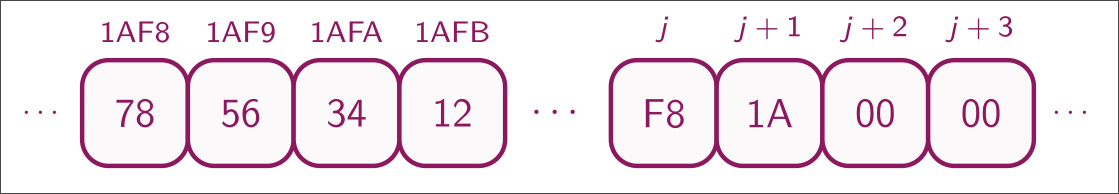
\includegraphics[scale=0.2]{2022-09-27-04:12:53.png} \newline
1AF8 now has a pointer in another place. \newline
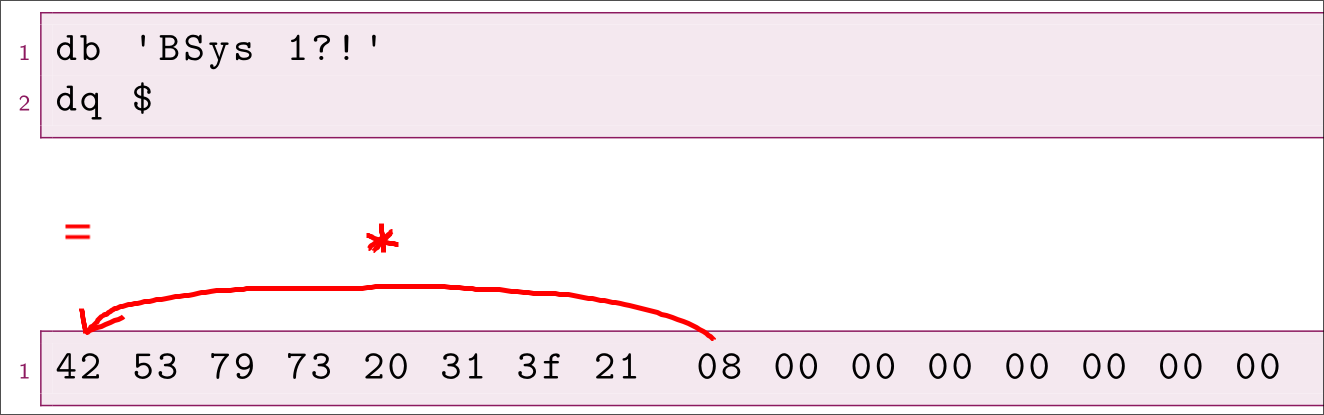
\includegraphics[scale=0.2]{2022-09-27-04:17:16.png}\newline
This would also produce the same result. Aka you can use labels before the operation.\newline
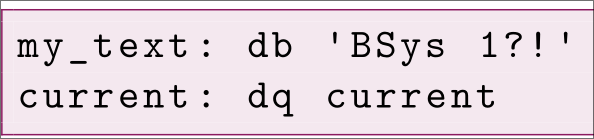
\includegraphics[scale=0.2]{2022-09-27-04:24:38.png}\\
\hline
A simple length calculation in assembly & \vspace{2mm} 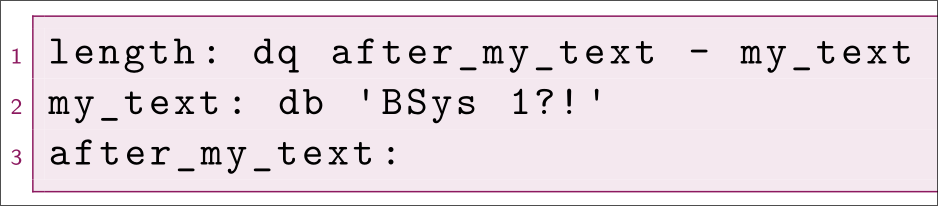
\includegraphics[scale=0.2]{2022-09-27-04:27:52.png}\newline 
First we define a label called length, but we can't calculate this yet as my\_text and after\_my\_text aren't defined yet.\newline
So we continue to the next line, here we write BSys 1?! and set the value of my\_text to 08 00 00 00 00 00 00.\newline
Then we define after\_my\_text with the value of the offset at this point, which is 0F 00 00 00 00 00 00 00.\newline
At last the length will have the value of 08 00 00 00 00 00 00 00, which is the length of BSys 1?!.\\
\hline
\textbf{\emph{Flat-Form Binaries vs Object-files}} & \textcolor{red}{The first is a simple binary of pure binary. Aka Machine-Code.}\newline
\textcolor{blue}{The second is the linked version with a symboltable to define labels.}\\
\hline
\textbf{\emph{Generate Object-file}} & \textbf{nasm -f elf64 prog.asm -o prog.o}\\
\hline
\textbf{\emph{Analyze Object-file}} & \textbf{objdump -t -d - Mintel prog.o}\newline
-t show symboltable \newline
-d disassemble\newline
-Mintel dissasemble code in intel format, aka show NASM format instead of GCC.\\
\hline
Assembly dumps in action & \vspace{2mm} 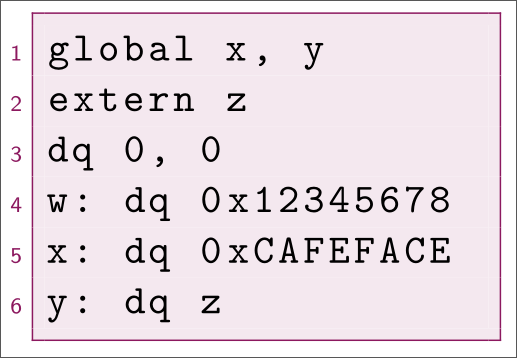
\includegraphics[scale=0.2]{2022-09-27-04:45:55.png} 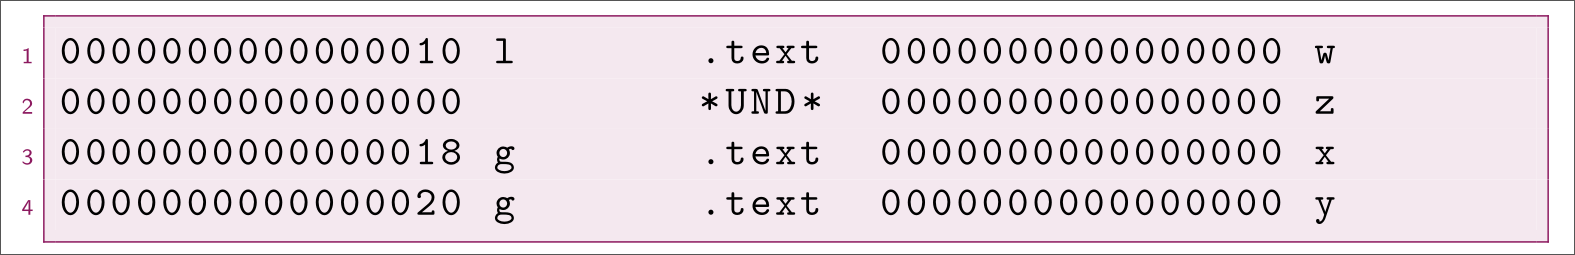
\includegraphics[scale=0.2]{2022-09-27-04:46:02.png}\newline
write 2 bytes aka a word to file. offset is now at 16, or 10 in hex.\newline
Now we use label w, which is at offset 10h, then we write 0x12345678 size 8h.\newline
label x, offset 18h, write 0xCAFEFACE size 8h.\newline
label y, offset 20h, write z, \textbf{\emph{but this is empty until compiled!}}
\\
\hline
\textbf{mov Target/Sink, Source} & 
\vspace{2mm}
\begin{itemize}
  \item copy from source into target
  \item after execution of operations, the source and target/sink have the same value
  \item \emph{\textbf{Target <- Source}}
\end{itemize}
Here an example: \newline
mov rax, eax \t --> move register to register (no memory access) \newline
mov rax, 0x4000 \t --> move constant into register (no memory access)\newline
mov rax, [eax] \t --> move memory address of value eax into rax (memory access!)\\
\hline
\textbf{mov rules} &
\vspace{2mm}
\begin{itemize}
  \item \emph{move eax, ebx} | move 32 bit into 32 bit // ok
  \item \emph{move eax, rbx} | move 64 bit into 32 bit // ERROR!
  \item mov [0x8000], rax | put content of memory \(8000_h\) ... \(8007_h\) to the content of rax
  \item mov [0x8000], 5 | put content of memory \(8000_h\) ... \(8007_h\) to 5
  \item \textbf{HOWEVER, you can't move from memory to memory!}
  \item \textcolor{red}{mov [0x8000], [0x9000] ERROR!!!!!}
  \vspace{-3mm}
\end{itemize}\\
\hline
\end{tabular}
\end{table}
\pagebreak
\begin{table}[h!]
\begin{tabular}{|m{0,2\linewidth}|m{0.755\linewidth}|}
\hline
Operand size with memory & 
\vspace{2mm}
\begin{itemize}
  \item 8 bit: mov al, [0x8000] | copy content of 1 byte to al
  \item 16 bit: mov ax, [0x8000] | copy content of 2 bytes to ax
  \item 32 bit: mov eax, [0x8000] | copy content of 4 bytes to eax
  \item 64 bit: mov rax, [0x8000] | copy content of 8 bytes to rax \newline
  \textcolor{red}{assembly copys as much as it can into the operand.}
  \vspace{-3mm}
\end{itemize}\\
\hline 
\textbf{\textcolor{teal}{Displacement and Base}}&\minipg{
\pic{2022-10-04-04:29:18.png}\newline
\textcolor{red}{\textbf{Displacement is the use of an address directly -> [0x8000]}}}
{\pic{2022-10-04-04:29:27.png}\newline
\textcolor{green}{\textbf{Base is the use of an address with a variable -> [rbx]}}}[0.4,0.4]\\
\hline
\textbf{\textcolor{teal}{Scaled Index}} &
[i * s]
\begin{itemize}
  \item Index i is a register
  \item Scale s is the constant 1,2,4 or 8 -> bytes!
  \item The address is i * s
  \item The index is therefore scaled
\end{itemize}
mov rcx, 0x1000 \newline
mov rax, [rcx * 8] // rcx multiplied by 8. Since rcs is 0x1000 -> 0x8000\newline
Or you can also write it like this:\newline
mov rbx , 0 x4000\newline
mov rcx , 0 x1000\newline
mov rax , [0 x2000 + rbx + rcx * 2]\newline
\\
\hline
\textbf{Hello World in assembly} &
\begin{lstlisting}
hello: db 'Henlo Birb' ;db something -> write your text
hello_length: equ $ - hello ;hello_length is equal to the current pointer minus hello

global _start         ; specifies the scope of a variable
_start:               ; like main in cpp
mov rax, 0x1          ; move system write instruction into register -> write instruction is 1
mov rdi, 0x1          ; specifies to write to the IO register 
mov rsi, hello        ; move text into write register
mov rdx, hello_length ; move write pointer to before rsi
syscall               ; call the os to do something

mov rax, 60           ; move system exit instruction into register -> 60
mov rdi, 0            ; ? exit code for string operation?
syscall               ; call the os to do something
\end{lstlisting}\\
\hline
\textbf{Instructions} & 
\vspace{2mm}\large
\begin{itemize}
\item mov rax, 1 \textcolor{teal}{//move the value 1 into rax, keep in mind that mov can hold other operations!}
\item equ rax, 1+1 \textcolor{teal}{//arithmic operation}
\item add z,   q  \textcolor{teal}{// z + q} 
\item sub z,   q  \textcolor{teal}{// z - q}
\item adc z,   q  \textcolor{teal}{// z + q + c (carry bit from previous calculation)}
\item sbb z,   q  \textcolor{teal}{// z - q - c (carry bit from previous calculation)}
\item neg z       \textcolor{teal}{// 0 - z ("zweierkomplement")}
\item inc z       \textcolor{teal}{// z++ }
\item dec z       \textcolor{teal}{// z-- }
\item mul z,      \textcolor{teal}{// multiply with implicit 2.operand }\newline
mul rbx -> RDX:RAX <-- RAX * RBX
\item imul z,   i  \textcolor{teal}{// signed equivalent for mul, z * i }
\item div z,      \textcolor{teal}{// divide with implicit 2.operand}\newline
div rbx  \newline
d = RDX:RAX\newline
RAX <-- RDX:RAX / RBX\newline
RDX <-- RDX:RAX mod RBX
\item shl z,   i  \textcolor{teal}{// z * \(2^i\)               --> shift}
\item shr z,   i  \textcolor{teal}{// z * \(2^{-i}\) z signed   --> shift}
\item sar z,   i  \textcolor{teal}{// z * \(2^{-i}\) z unsigned --> shift}
\item rol z,   i  \textcolor{teal}{// Left-Rotate i Bits }
\item ror z,   i  \textcolor{teal}{// Right-Rotate i Bits }
\end{itemize}
\, \newline
\textcolor{teal}{cmp: This instruction essentially does the same as sub rax, rbs, however,\newline
the difference is that sub will overwrite the rax value, cmp will not!\newline
\textbf{cmp will only set the flags!}}\newline
\\
\hline
NAND in Assembly & 
\begin{lstlisting}
mov rax,  [x] ; rax <- x
mov rbx,  [y] ; rbx <- y
and rax,  rbx ; rax <- x AND y
not rax       ; rax <- NOT ( x AND y )
mov [z], rax  ; z   <- NOT ( x AND y )
\end{lstlisting}\\
\hline
Size in Assembly & 
\textcolor{orange}{With certain instructions, the size can't be derived\newline
here we need to specify the size!}\newline
\begin{lstlisting}
not word [myvar] ; the word being the size
\end{lstlisting}\\
\hline
\end{tabular}
\end{table}
\pagebreak
\begin{table}[h!]
\section{Linker}
\begin{tabular}{|m{0,2\linewidth}|m{0.755\linewidth}|}
\hline
Movation & 
\vspace{2mm}
\begin{itemize}
  \item translate files
  \item \textbf{translate iteratively, only translate those that have changed!}
  \item \textbf{distribute development to many people!}
  \item \textbf{version control}
\vspace{-3mm}
\end{itemize}\\
\hline
Unlinked files in C C++ and assembly & \textcolor{red}{The UND is means that there is a not yet linked symbol!}\newline 
\pic{2022-10-04-04:41:27.png}\\
\hline
Partial Linking & 
\textbf{ld -r prog.o prog2.o -o prog3.o}  | This links our missing symbol from above!\newline
\pic{2022-10-04-04:44:56.png}\\
\hline
\textbf{Creation an executable} & 
\pic{2022-10-04-04:49:23.png}\newline
\begin{itemize}
  \item ld //the tool
  \item -e // flag for executable
  \item main // the entry point!
  \item my\_prog.o // the object file to use
  \item -o // outputflag
  \item my\_prog // the name of the executable to create
\vspace{-3mm}
\end{itemize}\\
\hline
\textbf{Syscall / End of a Program} & \minipg{ 
\begin{itemize}
  \item mov rax, 60 | \textbf{OS-Syscall exit code -> 60} |put 60 into rax
  \item rdi, 0 | \textbf{8 bit exit code} | exit code 0 aka successful
  \item syscall | \textcolor{red}{execute rax code -> exit!}
\vspace{-3mm}
\end{itemize}}
{\pic{2022-10-04-04:52:29.png}}[0.39,0.4]\\
\hline
\end{tabular}
\end{table}
\pagebreak
\begin{table}[ht!]
\section{C Toolchain}
\begin{tabular}{|m{0.977\linewidth}|}
\hline 
\minipg{
\textcolor{red}{The C Toolchain consists of:}\newline
\begin{itemize}
  \item \textcolor{teal}{C Preprocessor} 
  \item \textcolor{teal}{C Compiler} 
  \item \textcolor{teal}{Assembler} 
  \item \textcolor{teal}{Linker} 
\end{itemize}
}{
  C just like C++ has 3 parts:\newline
  \begin{itemize}
    \item \textcolor{teal}{Preprocessor} -> parts like \#include
    \item \textcolor{teal}{Base contructs} -> variables function etc inside one file and in the base language
    \item \textcolor{teal}{Standard libraries} -> additional function and types 
    \vspace{-3mm}
  \end{itemize}
}\\
\hline
\end{tabular}
\section{C Preprocessor}
\begin{tabular}{|m{0.2\linewidth}|m{0.755\linewidth}|}
\hline
1. Iteration & 
In the first iteration the preprocessor removes all comments from the code.\\
\hline
2. Iteration &
The preprocessor tokenizes the code, so the compiler has an easier time later on.\newline
\textcolor{teal}{Here are the possible tokens:}
\begin{itemize}
  \item \textcolor{teal}{Identifier}\newline
    starts with a-z or A-Z followed by letters, digits, or \_
  \item \textcolor{teal}{Preprocessor Number}\newline
    starts with a digit followed by digits, numbers, \_, ., or exponents
  \item \textcolor{teal}{String or Character literals}\newline
    String starts with ""\newline
    Character starts with ''\newline
    Escape character is \textbackslash
  \item \textcolor{teal}{Operations and punctuators}\newline
    \pic{2022-10-11-03:40:12.png}\newline
    \textcolor{orange}{The C preprocessor is greedy, it means that it will always take the biggest possible token}
  \item \textcolor{teal}{others}

\end{itemize}
\, \newline
\textcolor{orange}{The whitespaces, tabs and newlines seperate the tokens, however not all tokens need to be seperated, such as a+b.}\newline
\pic{2022-10-11-03:35:25.png}\\
\hline
3. Iteration & 
Here the C preprocessor simply \textbf{executes preprocessor directives} and \textbf{replaces macros} with code.\\
\hline
Function & Preprocessor handles such things as \#include \#define and more.\newline
They are simply used to put the code into one piece again, something that we humans are too dumb to do :P\\
\hline
\end{tabular}
\subsection{Preprocessor Commands:}
\begin{tabular}{|m{0.2\linewidth}|m{0.755\linewidth}|}
\hline
\#ifdef / \#ifndef \newline \#define \newline \#endif & These are used to check if things are already defined, or to define them. Either for checks to avoid double definition, or to check if debug is used -> ifdef DEBUG\\
\hline
Include differences & \#include <library> \textcolor{teal}{search in the system include directories!}\newline
\#include "library" \textcolor{teal}{search in the current working directory, \textbf{AND after that in the system includes}}\\
\hline
\#pragma once & This is used to automatically avoid double include statements. Aka if it is included already simply ignore any double includes. \\
\hline
\textbf{Cmake} & cmake -B build | this will define the directory to build in \newline cmake --build directory | this will build the system into this directory \newline cmake . | creates the CMakeFile and other files inside the specified director
\\
\hline
\textbf{Macros (simple object version)} & 
\#define XYZ 123 \newline
int x = XYZ compiles to int x = 123\newline 
\textcolor{orange}{Macros can't be a single character !}\\
\hline
\textbf{General Rule} & \emph{Only include what's necessary, don't just generalize includes to include everything!}\\
\hline
\end{tabular}
\section{C Compiler / Linker}
\begin{tabular}{|m{0.2\linewidth}|m{0.755\linewidth}|}
\hline
Commands &
\begin{itemize}
  \item gcc prog.c -o prog \textcolor{teal}{compile and link the prog.c with the ouput prog}
  \item gcc -c prog.c \textcolor{teal}{only compile the program -> prog.s as output}
  \item gcc -masm=intel -S prog.c \textcolor{teal}{only compile without assembling -> prog.o as output}
  \item gcc -E prog.c > prog.prep.c \textcolor{teal}{only run preprocessor commands -> prog.prep.c as output}
  \vspace{-3mm}
\end{itemize}\\
\hline
Function & 
\textcolor{orange}{\textbf{The compiler translates a pure c file (no preprocessor commands) to an assembly file}}\\
\hline
\end{tabular}
\end{table}
\begin{table}[ht!]
\begin{tabular}{|m{0.2\linewidth}|m{0.755\linewidth}|}
\hline
Translation example from C to Assembly &\pic{2022-10-11-04:26:03.png}\\
\hline
\textbf{\emph{Declaration}}
&
This only declares the variable, it does not have a predefined value -> undefined behavior!\newline
\begin{lstlisting}
exter int i;
extern char c;
\end{lstlisting}
\,\newline
\textcolor{red}{\textbf{PLEASE, note the \emph{extern} keyword}}\newline
\textcolor{orange}{This means that only a tag is declared, there is no memory allocation yet.\newline
Without extern the memory is allocated, this is as the extern expects the variable to be declared/defined somewhere else}\\
\hline
\textbf{\emph{Definition}}
&
This defines a variable with a set value.\newline
\begin{lstlisting}
int i = 5;
int a{5};
\end{lstlisting}
\\
\hline
\end{tabular}
\begin{tabular}{|m{0.2\linewidth}|m{0.3665\linewidth}|m{0.3665\linewidth}|}
\hline
Assembly vs C Declaration and Definition &
Assembly:\newline 
\begin{lstlisting}
my_var : dq 0 x4000
mov rax , [ my_var ]
\end{lstlisting}
\, \newline
C:\newline
\begin{lstlisting}
int my_var;
\end{lstlisting}
&
Assembly:\newline
\begin{lstlisting}
x : dd 15
\end{lstlisting}
\, \newline
C:\newline
\begin{lstlisting}
int x = 15;
\end{lstlisting}
\\
\hline
\end{tabular}
\begin{tabular}{|m{0.2\linewidth}|m{0.755\linewidth}|}
\hline
\textbf{static keyword} & 
\textcolor{red}{as there are no classes in C, the static keyword is used for something else\newline
This means that the variable can't be exported!!}\newline
\begin{lstlisting}
static int c = 5;
\end{lstlisting}
\, \newline
\pic{2022-10-11-11:12:14.png}\\
\hline
\textbf{Identifiers} & 
Identifiers are needed to format the output of \textcolor{teal}{printf} as a certain number/type.\newline
\begin{itemize}
\item \textcolor{teal}{Integer = \%d}
\item \textcolor{teal}{double = \%f}
\item \textcolor{teal}{}
\item \textcolor{teal}{}
\vspace{-3mm}
\end{itemize}\\
\hline
\end{tabular}
\subsection{Objects in C}
\begin{tabular}{|m{0.977\linewidth}|}
\hline
\textcolor{orange}{\textbf{C is not object oriented, objects are not the same as in C++}\newline
When we talk about objects in C, then we talk about any variable instance, for example an integer is an object.}\newline
\textcolor{teal}{Each object has some sort of value, for integer this is a number.}\newline
\textcolor{blue}{\textbf{In the end, an object is just an allocation of memory!}}\newline
The reason for this is that we once thought we might have a different way of storing things at some point\newline
Turns out this was wrong and we still use memory for storing everything.\\
\hline
\end{tabular}
\begin{tabular}{|m{0.2\linewidth}|m{0.755\linewidth}|}
\hline
Operations in C & 
\textcolor{orange}{C will enforce operand type equality, this means that it will try to cast to get this,\newline
or it will simply not work.}\\
\hline
Existence of types & 
Just like c++, after you compile C, it will no longer have types, just like assembly.\newline
Types only exist to make it easier to program.\\
\hline
\textbf{sizeof(T)}&
\textcolor{orange}{Each type has a size that you can check, however, this is compiler, OS and even architecture dependent!\newline This can therefore not be taken for granted.}\newline
\textcolor{red}{However, this is one of the reasons that C and C++ is so fast!}\\
\hline
\textbf{\textcolor{red}{minimum} size of variables}&
\vspace{2mm}
\begin{itemize}
  \item \textcolor{teal}{signed char} \(\geq\) 8 Bit
  \item \textcolor{teal}{short int} \(\geq\) 16 Bit
  \item \textcolor{teal}{int} \(\geq\) 16 Bit \(\geq\) short
  \item \textcolor{teal}{long int} \(\geq\) 32 Bit
  \item \textcolor{teal}{long long int} \(\geq\) 64 Bit
  \item \textcolor{teal}{void} no real value!
  \vspace{-3mm}
\end{itemize}\\
\hline
\end{tabular}
\end{table}
\pagebreak 
\begin{table}[ht!]
\begin{tabular}{|m{0.2\linewidth}|m{0.755\linewidth}|}
\hline
signed or unsigned & 
\textcolor{orange}{Just like in c++ you can write unsigned to get the max possible positive number.\newline
the default is signed, which has both negative and positive values!}\\
\hline
Other Types in C & 
\vspace{2mm}
\begin{itemize}
  \item \textcolor{teal}{Array-Types}
  \item \textcolor{teal}{Struct-Types}
  \item \textcolor{teal}{Union-Types}
  \item \textcolor{teal}{Pointer-Types}
  \item \textcolor{teal}{Function-Types}
  \vspace{-3mm}
\end{itemize}\\
\hline
Pointer types& 
\textcolor{orange}{\textbf{A pointer is just a number, it is an integer}}\newline
\textcolor{teal}{They simply \emph{point} to an address, this an be any address even another pointer address!}
\begin{lstlisting}
int num = 5;
int* nump; // pointer to int
int num2 = *nump; 
// dereference the pointer and assign the value of it to num2
int** numpp = &nump;
// create a pointer to a pointer with the address of nump
\end{lstlisting}
\\
\hline
Decimal,Octal and Hex & 
\vspace{2mm}
\begin{itemize}
  \item \textcolor{teal}{Decimal: 0..9 with \textbf{NO 0 at the start}} 
  \item \textcolor{teal}{Octal: 0..7 with a \textbf{leading 0}} 
  \item \textcolor{teal}{Hex: 0..F with \textbf{0x at the start}} 
  \item \textcolor{teal}{Suffix: the suffix specifies the type:}\newline
    l long,ll long long ,u unsigned,ul .. ,ull ..
  \vspace{-3mm}
\end{itemize}\\
\hline
Casts & 
\textcolor{orange}{Casts are just like in c++}\newline
\begin{lstlisting}
double ping = 5.5;
int pang = (int)ping;
\end{lstlisting}\\
\hline
Bitwise Operators & 
\vspace{2mm}
\begin{itemize}
  \item \textcolor{teal}{not: \(\tilde{} \) q}
  \item \textcolor{teal}{and: q \& p }
  \item \textcolor{teal}{or: q | p}
  \item \textcolor{teal}{or: q \^ p}
  \item \textcolor{teal}{or: q << p} left shift
  \item \textcolor{teal}{or: q >> p} right shift
\end{itemize}
\, \newline
\textcolor{teal}{Bitwise operators always return the same type we entered!}\newline 
\textcolor{orange}{Unlike assembly, you can't use rotate directly!} \\
\hline
Arithmic Operators& 
\vspace{2mm}
\begin{itemize}
  \item \textcolor{teal}{not: !q}
  \item \textcolor{teal}{and: q \&\& p}
  \item \textcolor{teal}{or: q || p}
  \item \textcolor{teal}{greater than: >}
  \item \textcolor{teal}{smaller than: <}
  \item \textcolor{teal}{greater than or equal: >=}
  \item \textcolor{teal}{smaller than or equal: <=}
\end{itemize}
\, \newline
\textcolor{red}{\textbf{The return type of these is int NOT bool!}}\newline
The reason for this is that C is a very old language and bool didn't exist when it was created.\\
\hline
\textbf{Imul vs Mul} & 
\textcolor{orange}{(C) In case of 2 unsigned integers, we should technically use the mul instruction,\newline
however, the compiler will often use the imul instruction instead as it is better for optimization!\newline
The reason for the imul usage, is that 2 negative numbers would result in the same operation as 2 regular numbers\newline 
therefore 2 normal numbers will result in the same operation!}\newline
\textcolor{red}{Important with imul the signed integers will be treated as negative! But AGAIN this does \textbf{NOT} matter!!!}\\
\hline
\textbf{Carry Flag} & 
\textcolor{orange}{The carry flag signifies the \textbf{overflow with unsigned integers!}}\newline
\textcolor{teal}{0001 + 1111 = 0000 AND CF = 1 -> 1 + 15 = 0 -> CF = 1}\\ 
\hline
\textbf{Overflow Flag} & 
\textcolor{orange}{The  overflow flag signifies the \textbf{overflow with signed integers!}}\newline
\textcolor{teal}{0111 + 0001 = 1000 -> 7 + 1 = -8 (only 3 bits are for data!! first bit is the signature!!)}\\
\hline
CF vs OF &
\textcolor{red}{The compiler can't distinguish between unsigned or signed for a number, this is why it always sets both flags, later on the compiler needs to use the right one.\newline
This means on overflow, both values are set and then later on the right flag will be used based on the variable!}\\
\hline
\textbf{FlagList} & 
\vspace{2mm}
\begin{itemize}
\item \textcolor{teal}{CF:} Carry Flag, overflow for unsigned integers 
\item \textcolor{teal}{OF:} Overflow Flag, overflow for signed integers
\item \textcolor{teal}{ZF:} Zero Flag, will be set when the result is 0
\item \textcolor{teal}{SF:} Sign Flag, is the highest bit of the result -> leftmost byte (little endian)
\item \textcolor{teal}{PF:} Parity Flag, set if the lowest byte has an even number of bits
\vspace{-3mm}
\end{itemize}\\
\hline
\textbf{Condition Codes (CC)} & 
\textcolor{orange}{Certain instructions will only be used when a combination of flags is given -> Condition Code}\newline
\textcolor{teal}{Example: condition "Above" -> CF = 0 AND ZF = 0}\newline
\textcolor{green}{List of CC:}\newline
\begin{tabular}{|ll|ll|}
\hline
\textcolor{teal}{A : Above }& \textcolor{teal}{ -> CF = 0 AND ZF = 0}&
\textcolor{teal}{AE: Above or Equal } & \textcolor{teal}{ -> CF = 0}\\
\textcolor{teal}{B : Below } & \textcolor{teal}{ -> CF = 1}&
\textcolor{teal}{BE: Below or Equal } & \textcolor{teal}{ -> CF = 1 AND ZF = 1}\\
\textcolor{teal}{E : Equal }& \textcolor{teal}{ -> ZF = 1}&
\textcolor{teal}{G : Greater }& \textcolor{teal}{ -> SF = OF = 0 AND ZF = 0}\\
\textcolor{teal}{GE: Greater or Equal }& \textcolor{teal}{ -> SF = OF}&
\textcolor{teal}{L : Less }& \textcolor{teal}{ -> SF != OF}\\
\textcolor{teal}{LE: Less or Equal }& \textcolor{teal}{ -> SF != OF AND ZF = 1}&
\textcolor{teal}{PE: Parity Even} & \textcolor{teal}{ -> PF =1}\\
\textcolor{teal}{PO: Parity Old } & \textcolor{teal}{ -> PF = 0}&
\textcolor{teal}{Z:  Zero}&\textcolor{teal}{ -> ZF = 1} \\
\end{tabular}
\\
\hline
\end{tabular}
\end{table}
\pagebreak
\begin{table}[ht!]
\begin{tabular}{|m{0.2\linewidth}|m{0.755\linewidth}|}
\hline
Jumps & 
\textcolor{orange}{This is essentially goto!}\newline
\begin{lstlisting}
jmp 230 ; moves 230 down 
jmp -230 ; moves 230 up
; We can also jump to labels!!!!
  mov eax, [x]
  cmp eax, 3
  jne label1 ; jump to label1 if eax not equal to 3
  mov eax, [y]
  
label1: 
  inc eax
\end{lstlisting}\\
\hline
Conditional Mov & 
\textcolor{orange}{cmovCC: mov if condition is met! \textbf{the cc stands for the code!}}\newline
\begin{lstlisting}
mov rax, [ux]
mov rbx, [uy]
cmp rax, rbx
cmove rcx, 5 ; move 5 into rcx if rax and rbx are equal!
\end{lstlisting}\\
\hline
Conditional JMP & 
\textcolor{orange}{jCC: jmp if condition is met! \textbf{the cc stands for the code!}}\newline
\begin{lstlisting}
cmp rax, rbx
je 230 ; move 230 down if rax and rbx are equal
\end{lstlisting}\\
\hline
Conditional SET &
\textcolor{orange}{setCC: set if condition is met! \textbf{the cc stands for the code!}}\newline
\begin{lstlisting}

\end{lstlisting}\\
\hline
If Else & 
\begin{lstlisting}
mov eax, [ux]
cmp eax, 2 
ja else_body ; jump to else statements if condition is met

jmp after_if ; will only be hit when condition at "ja" was false

else_body: 
; will only be hit if condition at "ja" was true
after_if:
; will be hit by everything
\end{lstlisting}\\
\hline
do while in assembly & 
\textcolor{red}{The do while loop is the worst loop possible according to the professor. lol}\newline
\begin{lstlisting}
loop: 
  dec rcx
  jnz loop ; if rcx not z, go to loop
\end{lstlisting}\\
\hline
While in assembly & 
\begin{lstlisting}
mov rcx, 23 
jmp condition 

loop: 
  ; body -> do something 
condition: 
  dec rcx 
  jnz loop ; move to loop if rcx not 0
\end{lstlisting}\\
\hline
For in assembly & 
\begin{lstlisting}
mov rcx, 0

loop: 

  inc rcx
condition: 
  cmp rcx 10
  jle loop
\end{lstlisting}\\
\hline
Pointer-Addition in assembly & 
\pic{2022-10-25-04:40:00.png}\newline
\textcolor{teal}{We can add additional bytes to a pointer. \newline
in C: int *p = 0x20; -> p+1 == 0x24 -> p+2 == 0x28\newline
or simply use the ++p for the same as p+1}
\, \newline
\begin{lstlisting}
extern int *begin; // defined somewhere else 
extern int *end;   // defined somewhere else 
int sum = 0;
for (int *p = begin; p != end; ++p) {
sum += *p; // same as regular for loop just with pointer instead
 ;// then dereference the pointer here to get the value 
 ;// warning, if you go beyong what you should -> undefined behavior, likely segmentation fault!
}
\end{lstlisting}
\\
\hline

\hline

\hline
\end{tabular}
\end{table}
\pagebreak
\begin{table}[ht!]
\begin{tabular}{|m{0.2\linewidth}|m{0.755\linewidth}|}
\hline

\hline

\hline

\hline

\hline

\hline

\hline

\hline

\hline

\hline

\hline
\end{tabular}
\end{table}
\pagebreak
\begin{table}[ht!]
\begin{tabular}{|m{0.2\linewidth}|m{0.755\linewidth}|}
\hline

\hline

\hline

\hline

\hline

\hline

\hline

\hline

\hline

\hline

\hline
\end{tabular}
\end{table}
\pagebreak
\begin{table}[ht!]
\begin{tabular}{|m{0.2\linewidth}|m{0.755\linewidth}|}
\hline

\hline

\hline

\hline

\hline

\hline

\hline

\hline

\hline

\hline

\hline
\end{tabular}
\end{table}
\end{document}
